\documentclass{standalone}
\usepackage{tikz}
\usepackage{verbatim}
\begin{document}
\pagestyle{empty}
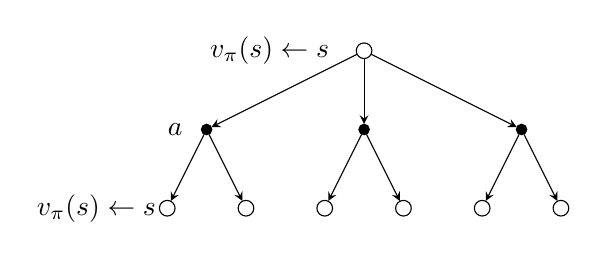
\begin{tikzpicture}

  % The graphic
  \node[draw,circle,scale=0.6] (s) at (0,0) {};
  \node at (-1.2, 0) {$v_{\pi}(s)\leftarrow s$};
  \foreach \x in {-2, 0, 2} {
      \node[draw,circle,fill,scale=0.4] (b\x) at (\x, -1) {};
      \node[draw,circle,scale=0.6] (l\x) at (\x-.5,-2) {};
      \node[draw,circle,scale=0.6] (r\x) at (\x+.5,-2) {};
      \draw[-stealth] (s) -- (b\x);
      \draw[-stealth] (b\x) -- (l\x);
      \draw[-stealth] (b\x) -- (r\x);
  }
  % \node at (0.2, -0.5) {$\pi$};
  \node at (-2.4, -1.) {$a$};
  % \node[below = 2mm of b1] {$p$};
  \node at (-3.4, -2.) {$v_{\pi}(s)\leftarrow s$};
\end{tikzpicture}
\end{document}